%%%%%%%%%%%%%%%%%%%%%%%%%%%%%%%%% Hauptteil %%%%%%%%%%%%%%%%%%%%%%%%%%%%%%%%%%

\chapter{Theoretischer Hintergrund}
\label{chap:background}

\section{Beispielkapitel}

\subsection{Referenzen und Fußnoten}

Dies ist eine Quellenangabe \citep{Pernul1994}. Man kann auch auf mehrere Arbeiten verweisen \citep{Pernul1994, pernul2009datenbanken}. Quellen werden in der Datei \textit{References.bib} gespeichert und können z.B. mit Mendeley\protect{\footnote{\url{https://www.mendeley.com}}} oder JabRef\protect{\footnote{\url{https://www.jabref.org/}}} verwaltet werden. Wenn etwas wörtlich zitiert werden soll, kann einfach
\textbf{\textbackslash enquote,} verwendet werden: \enquote{Dies ist ein Zitat}. So werden die Anführungszeichen immer richtig gesetzt. \par\smallskip


\subsection{Verwendung von Abkürzungen}

Die automatische Erstellung des Abkürzungsverzeichnisses ist ebenfalls sehr nützlich. Abkürzungen können in main.tex definiert werden. Zum Beispiel die Abkürzung \ac{SaaS}, wird so definiert, dass sie bei ihrer ersten Verwendung im Abkürzungsverzeichnis erscheint. Abkürzungen müssen konsistent verwendet werden, sobald sie eingeführt sind. Nicht jede Verwendung einer Abkürzung muss mit dem Befehl \verb+\ac{}+ verlinkt werden. Wenn jedoch viele Seiten zwischen der Verwendung einer Abkürzung liegen, kann ein Hyperlink für den Leser hilfreich sein.


\subsection{Aufzählungen}
In Latex gibt es zwei Arten von Aufzählungen, nummerierte Listen (\textbf{enumerate}):
\begin{enumerate}
    \item Punkt 1
    \item Punkt 2
    \item Punkt 3
\end{enumerate}

und umnummerierte Listen (\textbf{itemize}):

\begin{itemize}
    \item Punkt 1
    \item Punkt 2
    \item Punkt 3
\end{itemize}


\subsection{Abbildungen}
\label{sec:figures}

Die Größe von Abbildungen kann an die Textbreite angepasst werden. Abbildung~\ref{fig:Fig1} hat die volle Textbreite, Abbildung~\ref{fig:Fig2} 30\% davon.

\begin{figure} [!htb]
  \centering
  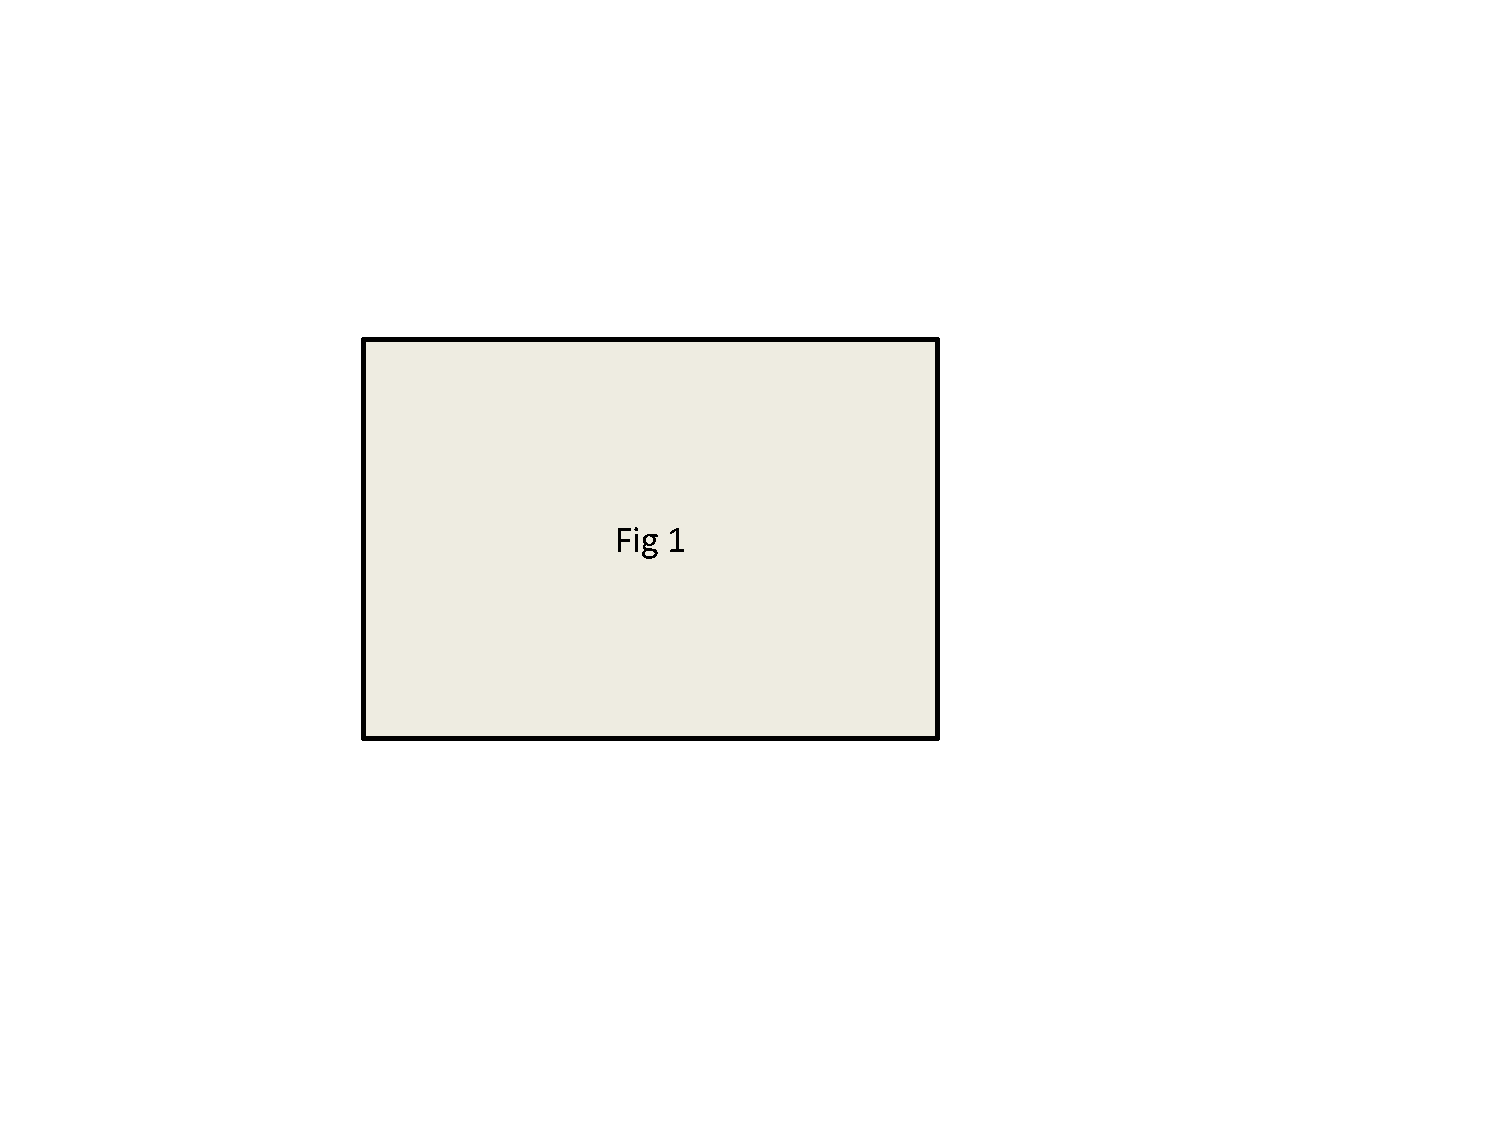
\includegraphics[width=\textwidth]{Fig1.pdf}
  \caption{Beispielhafte Abbildung.}
  \label{fig:Fig1}
\end{figure}


\begin{figure} [!htb]
  \centering
  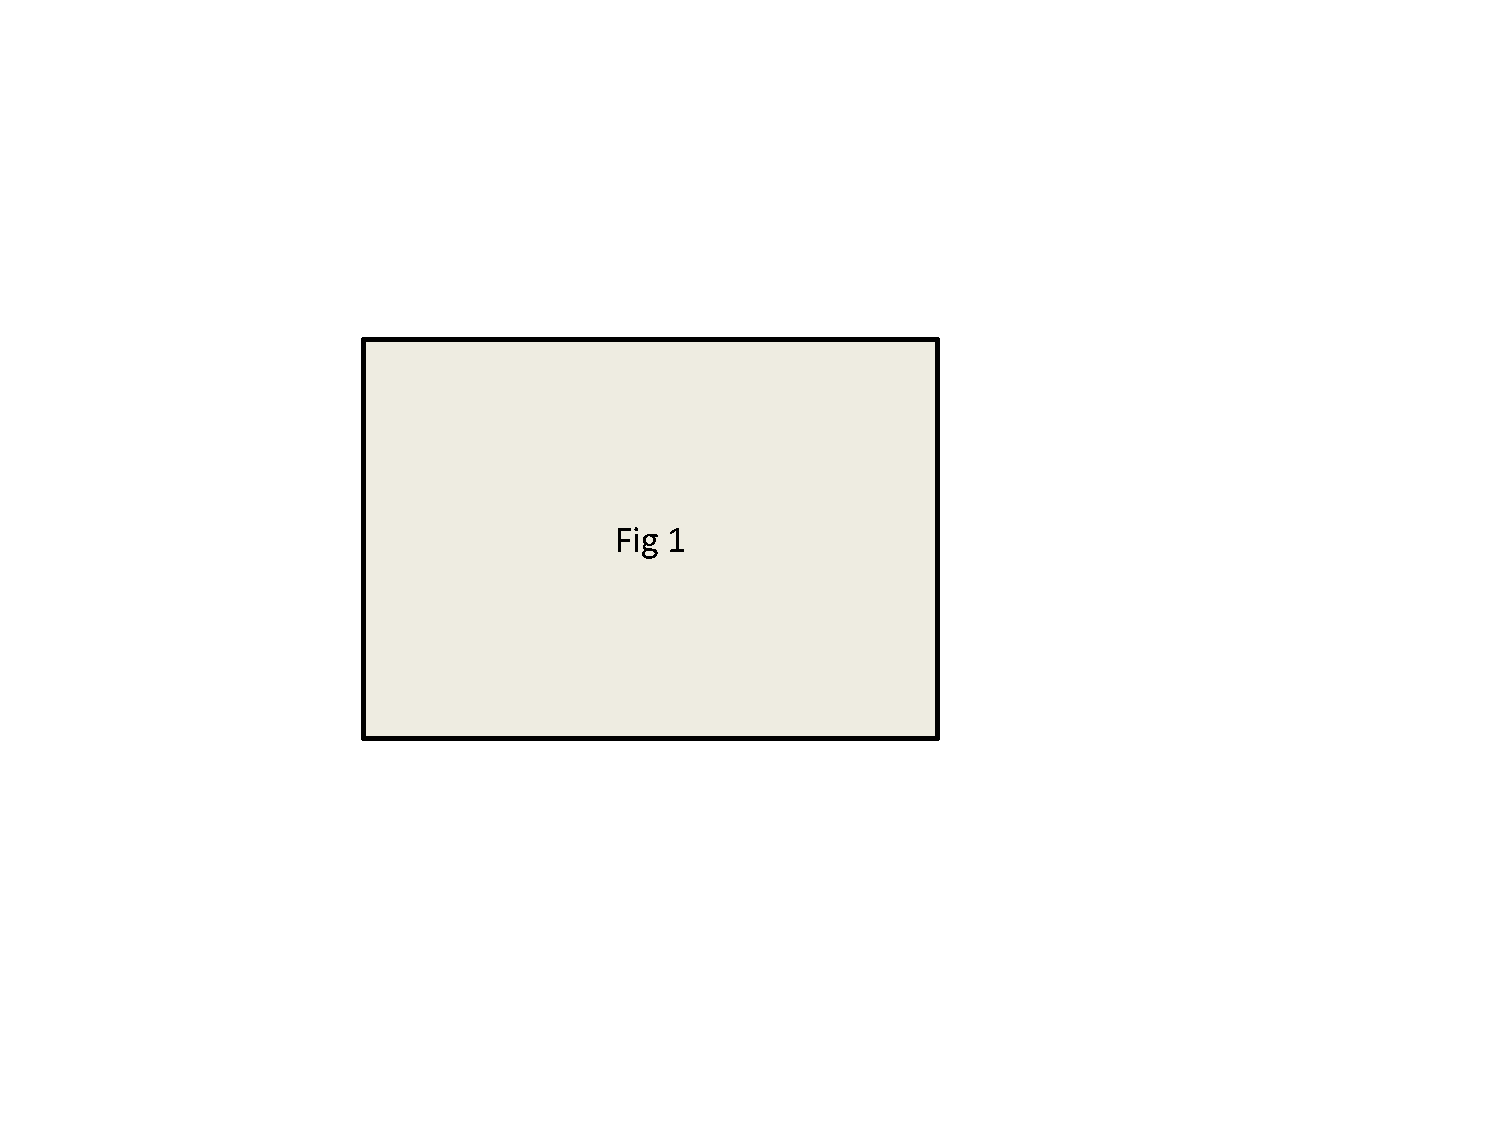
\includegraphics[width=0.3\textwidth]{Fig1.pdf}
 \caption{Beispielhafte kleinere Abbildung.}
  \label{fig:Fig2}
\end{figure}

\subsection{Tabellen}
\label{sec:tables}

In diesem Abschnitt ist ein Beispiel für eine Tabelle. Die Beschriftung von Tabellen befindet sich -- im Gegensatz zu Abbildungen -- immer oberhalb der Tabelle.

\begin{table} [h]
\centering
\caption{Beispielbeschriftung.}
\label{tab:feedback}
\begin{tabular}{lccc}
\toprule
\textbf{Bedingung} & \textbf{Mittelwert} & \textbf{Median} & \textbf{Standardabweichung} \\
\midrule
Wert 1 & 4.40 & 5 & 0.75 \\
Wert 2 & 4.35 & 4 & 0.72 \\
Wert 3 & 4.10 & 4 & 0.78 \\
Wert 4 & 4.23 & 4 & 0.72 \\
Wert 5 & 4.14 & 4 & 0.79 \\
\bottomrule
\end{tabular}
\end{table}








\subsection{Referenzen}

Der folgende Satz veranschaulicht die Verwendung von Referenzen. In Unterabschnitt~\ref{sec:figures}) wurde erklärt, wie man Abbildungen in \LaTeX verwendet, z. B. Abbildung~\ref{fig:Fig1}. Auf jede Tabelle, Abbildung oder Auflistung, die verwendet wird, muss mindestens einmal im Text Bezug genommen werden.

\subsection{Listings/Codebeispiele}

\lstset{language=JAVA, breaklines=true, tabsize=2}
\lstinputlisting[caption=HelloWorld,
label=lst:HelloWorld]{listings/HelloWorld.java}



\begin{landscape}

Seite im Querformat, z. B. für größere Abbildungen oder Tabellen; Fußzeile bleibt im Hochformat.

\end{landscape}




%%%%%%%%%%%%%%%%%%%%%%%%%%%%%%%%%%%%%%%%%%%%%%%%%%%%%%%%%%%%%%%%%%%%%%%%%%%%%%
